\documentclass{article}

%............Inicia Preambulo.......................
\usepackage{graphicx}
\usepackage{float}
\usepackage[utf8]{inputenc}
\usepackage[shortlabels]{enumitem}
\usepackage{textcomp}
\usepackage{multicol}
\usepackage{caption}
\usepackage[spanish]{babel}
\usepackage[total={17.5cm, 23cm}, top=2cm, left=2cm]{geometry}
\usepackage{esvect}
\usepackage[font=footnotesize]{caption}

\spanishdecimal{.}
\parindent 0cm

%.............Fin de Preambulo........................

\begin{document}

\begin{center}
{\Large \textbf{Universidad Autónoma de Coahuila}}
\end{center}

\begin{center}
{\large Facultad de Ciencias Físico-Matemáticas}
\end{center}

%Materia
\begin{center}
{\large Metodos Numericos}
\end{center}

%Título
\begin{center}
{\large Metodo de la Secante}
\end{center}

%Fecha
\begin{center}
{\large 29 de Noviembre del 2019}
\end{center}

%Autor
\begin{center}
{\large José Antonio Olveda García}
\end{center}

\vspace{5mm}

\begin{multicols}{2}

\section{Objetivo}
\label{sec:obj}
  Mostrar la utilidad del buscador de raices de polinomios por medio del metodo de la secante, asi como las ventajas y desventajas que este pueda presentar

\section{Introduccion}
\label{sec:Intro}
El metodo de la secante se basa en la formula de Newton-Raphson, pero evita el calculo de la derivada.

\section{Metodologia}
\label{sec:Met}
El principal inconveniente del método de Newton estriba en que requiere conocer el valor de la primera derivada de la función en el punto. Sin embargo, la forma funcional de f(x) dificulta en ocasiones el cálculo de la derivada. En estos casos es más útil emplear el método de la secante.
El método de la secante parte de dos puntos (y no sólo uno como el método de Newton) y estima la tangente (es decir, la pendiente de la recta) por una aproximación de acuerdo con la expresión:
\begin{equation}
f'(x_{0})=\frac{f(x_{1})-f(x_{0})}{x_{1}-x_{0}}
\end{equation}
Sustituyendo esta expresión en la ecuación del método de Newton, obtenemos la expresión del método de la secante que nos proporciona el siguiente punto de iteración:
\begin{equation}
x_{2}=x_{0}-\frac{x_{1}-x_{0}}{x_{1}-x_{0}} f(x_{0})
\end{equation}
En la siguiente iteración, emplearemos los puntos x1 y x2para estimar un nuevo punto más próximo a la raíz de acuerdo con la ecuación 2. En la figura 1 se representa geométricamente este método.
\begin{figure}[H]
\centering
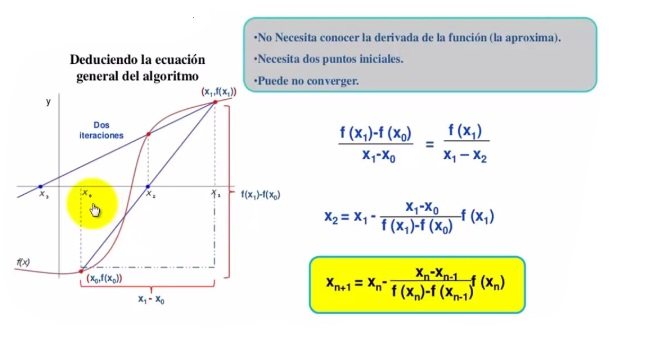
\includegraphics[scale=.375]{Secante.jpg}
\caption{Representacion geometrica del metodo de la secante} 
\end{figure}
El metodo de la secante es muy rápido y eficiente ya que la convergencia es de tipo cuadrático (el número de cifras significativas se duplica en cada iteración). Sin embargo, la convergencia depende en gran medida de la forma que adopta la función en las proximidades del punto de iteración. En la figura (7) se muestran dos situaciones en las que este método no es capaz de alcanzar la convergencia (figura (7a)) o bien converge hacia un punto que no es un cero de la ecuación 
\section{Ejemplo}
\label{sec:Ejem}
Resuelva el siguiente polinomio por medio de la regla falsa.
\begin{center}
$2x^{4}-5^{2}+x $ en el intervalo $[1,3.5]$
\end{center}
Evaluando obtenemos los siguientes valores
\\
$f_{a}=-2$ 
\\
$f_{b}=242.3$
\\
$x_{a}=1$
\\
$x_{b}=3.5$
Aplicando la regla de la secante obtenemos que el punto de la primera aproximacion es de 
$c=4.502$
Realizando la multiplicacion entre las funciones evaluadas en a y c, obtenemos 
\begin{center}
$-2*4.502=-9.004$
\end{center}
Por lo tanto se extiende la regla ahora con un nuevo intervalo, siendo de $[4,502,3.5]$, volviendo a realizar la regla falsa obtenemos un valor de $c=2.9$, extiendose la comprobacion has $n$ iteraciones deseadas.
Graficado por medio de Geogebra obtenemos una de sus raices la cual es $x=1.674$

\section{Ventajas y Desventajas}
\textbf{Ventajas}
\\
1. se puede aplicar cuando la funcion f(x) es demasiado compleja como para obtener su derivada
\\
2. No es tan complicado de programar.
\\
\\
\textbf{Desventajas}
\\
1. Su velocidad de convergencia es menor que la de otros metodos como Newton-Raphson.
\\
2. La convergencia de dicho metodo no asegura si la primera aproximacion a la raiz no es lo suficientemente cercana a ella  
\section{Implementacion del programa}
\label{sec:Imp}
El metodo de la secante al ser tan similar al metodo de regla falsa y biseccion, obtendran similitudes al encontrar las raices de las aproximaciones estimadas
observando la figura obtenemos que la raiz estimada efectivamente es de 1.67
\begin{figure}[H]
\centering
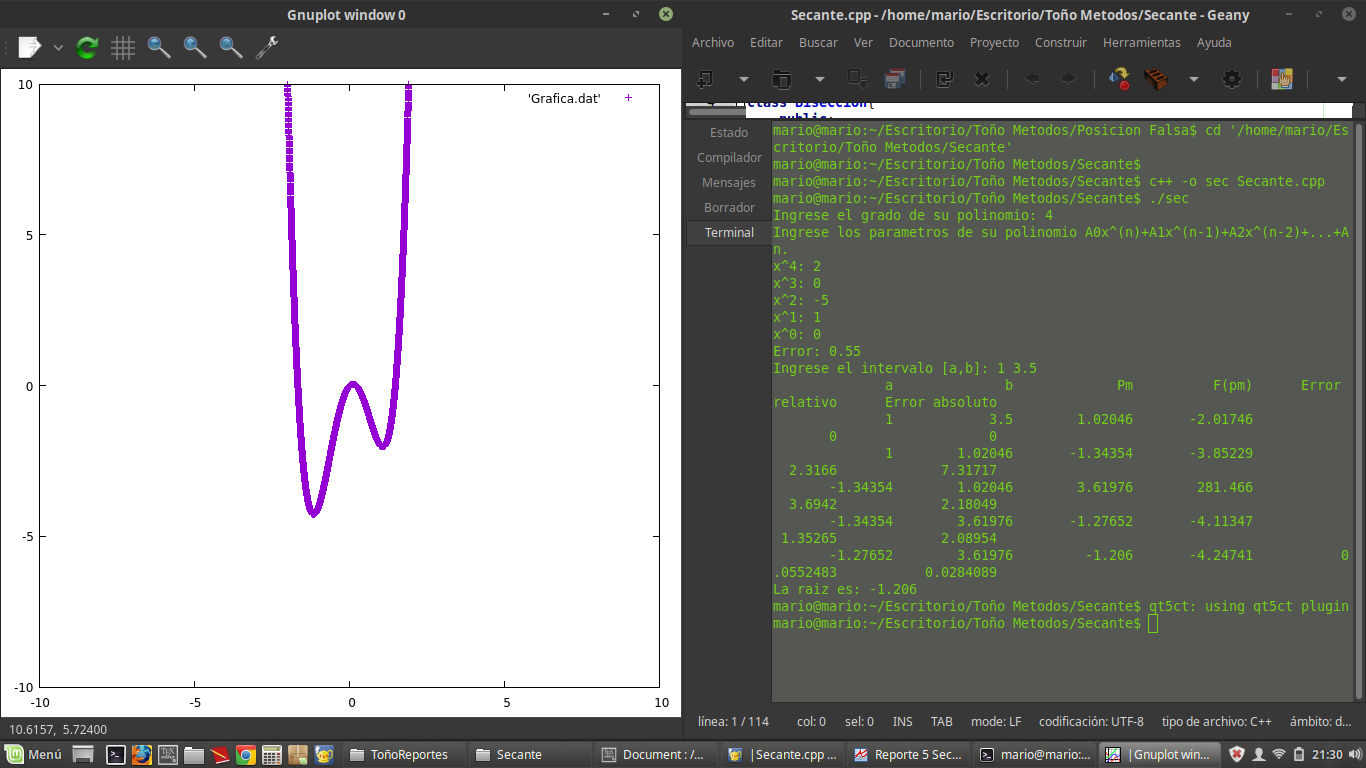
\includegraphics[scale=.125]{Secante.png}
\caption{Programa de la secante designado con el ejemplo anterior}
\end{figure}



\end{multicols}

\end{document}
